\documentclass[pdf]{beamer}

\mode<presentation>{}

%% Preamble
\usetheme{Madrid}
\usecolortheme{seahorse}
\usefonttheme{professionalfonts}

\setbeamertemplate{section in toc}{\inserttocsectionnumber.~\inserttocsection}
\setbeamertemplate{subsection in toc}{%
  \hspace{1.2em}{\color{blue}\rule[0.3ex]{3pt}{3pt}}~\inserttocsubsection\par}
\setbeamertemplate{itemize items}{%
  \color{blue}\rule[0.3ex]{3pt}{3pt}}

\usepackage{minted}

%% Hide syntax errors in minted
\AtBeginEnvironment{minted}{%
  \renewcommand{\fcolorbox}[4][]{#4}}

%% Set minted to remove preceeding space and set font size
\setminted[]{fontsize=\footnotesize,autogobble}

\usepackage{dirtree}
\usepackage{hyperref}

\hypersetup{
  colorlinks=true,
  linkcolor=black,
  urlcolor=cyan
}

\usepackage{graphicx}
\graphicspath{ {images/} }

\usepackage{etoolbox}

%% Remove extra spacing between sections in the table of contents
\makeatletter
\patchcmd{\beamer@sectionintoc}{\vskip1.5em}{\vskip0em}{}{}
\makeatother

\AtBeginSection[]
{
  \begin{frame}{Table of Contents}
    \tableofcontents[currentsection,hideothersubsections]
  \end{frame}
}

\AtBeginSubsection[]{
  \begin{frame}
    \vfill
    \centering
    \begin{beamercolorbox}[sep=8pt,center,shadow=true,rounded=true]{title}
    \usebeamerfont{title}\insertsubsectionhead\par%
    \end{beamercolorbox}
    \vfill
  \end{frame}
}

\title{Building a Blogging System}
\subtitle{with Haskell and Yesod}
\author{Gavin Whelan}

\begin{document}

%% title frame
\begin{frame}
  \titlepage
\end{frame}

\begin{frame}{About Me}
  IU Computer Science Graduate\\
  LambdaConf Hunger Prevention Manager\\
  \\
  My site: \href{https://ambientmemory.com}{ambientmemory.com}\\
  GitHub: \href{https://github.com/gavwhela}{@gavwhela}\\
  \\
  CTO Whiteboard Dynamics LLC\\
  Company site: \href{https://whiteboarddynamics.co}{whiteboarddynamics.co}\\
\end{frame}

\begin{frame}{Attributions}
  This presentation uses resources from the Yesod Book,\\
  \url{https://github.com/yesodweb/yesodweb.com-content}\\
  \url{http://www.yesodweb.com/book}\\
  \\
  as well as the yesod-postgres template.\\
  \href{https://github.com/commercialhaskell/stack-templates/blob/master/LICENSE}{MIT License}\\
\end{frame}

\section{Basic Background}
\subsection{Language Extensions}
\begin{frame}[fragile]{Overloaded Strings}
  \begin{minted}[frame=single]{haskell}
    class IsString a where
        fromString :: String -> a
  \end{minted}
  \pause
  \vspace{1em}
  Without OverloadedStrings
  \begin{minted}[frame=single]{haskell}
    "Literal String" :: String
    "Literal String" :: [Char]
  \end{minted}
  \pause
  \vspace{1em}
  With OverloadedStrings
  \begin{minted}[frame=single]{haskell}
    {-# LANGUAGE OverloadedStrings #-}
    "Literal String" :: IsString a => a
  \end{minted}
\end{frame}

\begin{frame}[fragile]{Type Families}
  \begin{minted}{haskell}
    {-# LANGUAGE TypeFamilies #-}
    import Data.Word (Word8)
    import qualified Data.ByteString as S
    
    class SafeHead a where
        type Content a
        safeHead :: a -> Maybe (Content a)
    
    instance SafeHead [a] where
        type Content [a] = a
        safeHead [] = Nothing
        safeHead (x:_) = Just x
    
    instance SafeHead S.ByteString where
        type Content S.ByteString = Word8
        safeHead bs
            | S.null bs = Nothing
            | otherwise = Just $ S.head bs
  \end{minted}
\end{frame}

\begin{frame}[fragile]{Template Haskell}
  \begin{minted}{haskell}
    {-# LANGUAGE TemplateHaskell #-}
    
    -- | Template Haskell (TH) is Haskell's approach to code
    -- generation. Yesod uses TH to reduce boilerplate. Code from
    -- before a TH splice cannot refer to code within the TH, or what
    -- follows.

    $(templateHaskellFunction arg1 arg2)

    -- | Or at the top level
    templateHaskellFunction arg1 arg2
  \end{minted}
\end{frame}

\begin{frame}[fragile]{QuasiQuotes}
  \begin{minted}{haskell}
    {-# LANGUAGE QuasiQuotes #-}
    
    -- | QuasiQuotes (QQ) allows arbitrary content to be taken inline
    -- in Haskell code and processed, generating Haskell code as TH does.

    -- | The name of the quasi-quoter is given between the opening
    -- bracket and the first pipe. The quasi-quoted region is closed
    -- with |]

    [hamlet|<p>This is quasi-quoted Hamlet.|]
  \end{minted}
\end{frame}

\subsection{Hello World}
\begin{frame}[fragile]{Hello World}
  \begin{minted}{haskell}
    {-# LANGUAGE OverloadedStrings #-}
    {-# LANGUAGE QuasiQuotes       #-}
    {-# LANGUAGE TemplateHaskell   #-}
    {-# LANGUAGE TypeFamilies      #-}
    import Yesod

    data HelloWorld = HelloWorld

    mkYesod "HelloWorld" [parseRoutes|
    / HomeR GET
    |]

    instance Yesod HelloWorld

    getHomeR :: Handler Html
    getHomeR = defaultLayout [whamlet|Hello World!|]

    main :: IO ()
    main = warp 3000 HelloWorld
  \end{minted}
\end{frame}

\begin{frame}{Hello World: Result}
  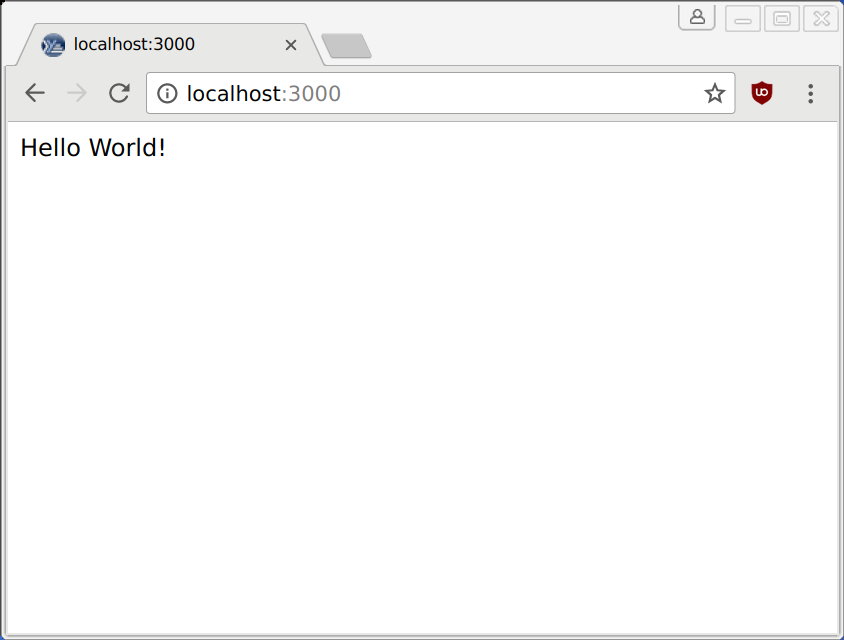
\includegraphics[width=\textwidth,height=0.8\textheight,keepaspectratio]{example}
\end{frame}

\section{Set up Codio \& Dive into an exercise}

\subsection{Codio}
\begin{frame}{Setting up Codio}
  Sign in to Codio \\

  Join the class \\

  Enter the first unit \\

  Should see readme \\
\end{frame}

\subsection{First Exercise}
\begin{frame}[fragile]{First Exercise}
  \begin{minted}{haskell}
    {-# LANGUAGE OverloadedStrings, QuasiQuotes #-}
    {-# LANGUAGE TemplateHaskell, TypeFamilies  #-}
    import Yesod

    data Links = Links

    mkYesod "Links" [parseRoutes|
    /      HomeR  GET
    /page1 Page1R GET
    /page2 Page2R GET
    |]

    instance Yesod Links

    getHomeR  = defaultLayout [whamlet|<a href=@{Page1R}>Go to page 1!|]
    getPage1R = defaultLayout [whamlet|<a href=@{Page2R}>Go to page 2!|]
    getPage2R = defaultLayout [whamlet|<a href=@{HomeR}>Go home!|]

    main = warp 3000 Links
  \end{minted}
\end{frame}

\subsection{What did we do?}

\begin{frame}{Congratulations!}
  Congratulations, you've just added a new page to a Yesod application!\\
  \\
  So far you've already used:\\
  \begin{itemize}
  \item Monads (hopefully you weren't scared of those)
  \item Shakespearean Templating
  \item Routing DSL
  \item Typesafe URLs
  \item Handlers
  \item Quasi-Quoters
  \item And more!
  \end{itemize}
\end{frame}

\section{Content Creation}
\subsection{Shakespearean Templating}
\begin{frame}{Shakespearean Templating}
  General purpose templating languages\\
  \\
  \begin{tabular}{ l l }
    Hamlet  & (HTML)\\
    Lucius  & (CSS)\\
    Cassius & (CSS)\\
    Julius  & (JavaScript)\\
  \end{tabular}
\end{frame}

\begin{frame}[fragile]{Interpolation}
  \begin{tabular} { l l }
    \mintinline{haskell}{#{myVar}}                               & Variable interpolation \\
    \pause
    \mintinline{haskell}{@{HomeR}}                               & URL interpolation \\
    \pause
    \mintinline{haskell}{@?{(HomeR, [("token", validateToken)]}} & $\uparrow$ With query parameters \\
    \pause
    \mintinline{haskell}{^{footer}}                              & Template Embedding\\
  \end{tabular}
\end{frame}

\begin{frame}{Hamlet}
  \begin{itemize}
  \item<1-> Whitespace based, no closing tags\\
  \item<2-> Interpolations\\
  \item<3-> Quality of life improvements\\
  \item<4-> Embedded logic, looping, and pattern matching \\
  \item<5-> Optional attributes\\
  \end{itemize}
\end{frame}

\begin{frame}[fragile]{Hamlet}
  \begin{minted}{HTML}
    $doctype 5
    <html>
        <head>
            <title> <a href=@{HomeR}> #{pageTitle} - My Site </a>
            <link rel=stylesheet href=@{Stylesheet}>
        <body #body>
            <h1 .page-title>#{pageTitle}
            <p>Here is a list of your friends:
            $if null friends
                <p>Sorry, I lied, you don't have any friends.
            $else
                <ul>
                    $forall Friend name age <- friends
                        <li>#{name} (#{age} years old)
  \end{minted}
\end{frame}

\begin{frame}[fragile]{Template interpolation}
  \begin{minted}{Haskell}
    wrapper :: HtmlUrl a -> HtmlUrl a
    wrapper content =
      [hamlet|
          <html>
              <head>
                  <title> My Site
              <body>
                ^{content}
      |]

    content :: HtmlUrl a
    content =
      [hamlet|
        <h1> Welcome
        <p> This is the content hamlet!
      |]
  \end{minted}
\end{frame}

\begin{frame}[fragile]{More Embedded Logic}
  Attributes:\\
  \begin{minted}[frame=single]{HTML}
    <input type=checkbox :isChecked:checked>
    <p :isRed:style="color:red">
  \end{minted}
  \pause
  Maybe values:\\
  \begin{minted}[frame=single]{HTML}
    $maybe name <- maybeName
      <p>Your name is #{name}
    $nothing
      <p>I don't know your name.
  \end{minted}
  \pause
  \begin{minted}[frame=single]{HTML}
    $maybe Person firstName lastName <- maybePerson
      <p>Your name is #{firstName} #{lastName}
  \end{minted}
\end{frame}

\begin{frame}[fragile]{More Embedded Logic}
  Pattern matching:\\
  \begin{minted}[frame=single]{HTML}
    $case foo
      $of Left bar
        <p>It was left: #{bar}
      $of Right baz
        <p>It was right: #{baz}
  \end{minted}
  \pause
  With:\\
  \begin{minted}[frame=single]{HTML}
    $with foo <- (long ugly) expression that $ should only $ happen once
      <p>But I'm going to use #{foo} multiple times. #{foo}
  \end{minted}
\end{frame}

\begin{frame}{Lucius}
  \begin{itemize}
  \item<1-> Intended to be a superset of CSS\\
  \item<2-> Nested blocks\\
  \item<3-> Variable definitions\\
  \item<4-> Mixins\\
  \end{itemize}
\end{frame}

\begin{frame}[fragile]{Lucius}
  \begin{minted}{CSS}
    @textcolor: #494949;                      /* Variable definition */
    body {
        color: #{textcolor};                  /* Variable interpolation */
        font-size: 16px;
    }
    .footer {
        background: url(@{BackgroundImageR}); /* URL interpolation */
        height: 150px;
        text-align: center;
        > .container {                        /* Nested block */
            padding: 45px 0 0 0;
        }
        p {
            margin-top: 45px;
            margin-bottom: 0px;
        }
    }
  \end{minted}
\end{frame}

\begin{frame}[fragile]{Cassius}
  Just Lucius, but whitespace instead of brackets and semicolons.\\
  You don't see this used too much.\\
  \begin{minted}[frame=single]{CSS}
    @textcolor: #494949
    body
        color: #{textcolor}
        font-size: 16px
    .footer
        background-image: url(@{BackgroundImageR})
        height: 150px
        text-align: center
        > .container
            padding: 45px 0 0 0
        p
            margin-top: 45px
            margin-bottom: 0px
  \end{minted}
\end{frame}

\begin{frame}[fragile]{Julius}
  Simplist of the three\\
  \pause
  Performs no transformations other than allowing the forms of interpolation\\
  \pause
  \begin{minted}[frame=single]{Javascript}
    $(function(){
        $("section.#{sectionClass}").hide();
        $("#mybutton").click(function(){
            document.location = "@{SomeRouteR}";
        });
        ^{addBling}
    });
  \end{minted}
\end{frame}

\begin{frame}[fragile]{QuasiQuoters}
  \begin{minted}{haskell}
    [hamlet| <h1>My Title |]
    [lucius| h1 { color: green } |]
    [julius| alert("Hi") |]
  \end{minted}
  \pause
  Wait a minute, what was that whamlet Quasi-Quoter?
\end{frame}

\subsection{Widgets}
\begin{frame}{Widgets}
  Yesod's solution to modular and composable web elements. \\
  Each widget has these components:\\
  \begin{itemize}
  \item<1-> The title
  \item<2-> External stylesheets
  \item<2-> External Javascript
  \item<3-> CSS declarations
  \item<3-> Javascript code
  \item<4-> Arbitrary \textless head\textgreater\ content
  \item<4-> Arbitrary \textless body\textgreater\ content
  \end{itemize}
\end{frame}

\begin{frame}[fragile]{Widget Monad}
  Widgets can be composed monadically.
  \begin{minted}[frame=single,escapeinside=??]{haskell}
    myWidget1 = do
      toWidget [hamlet|<h1>My Title|]
      toWidget [lucius|h1 { color: green } |]
    ?\pause?
    myWidget2 = do
      setTitle "My Page Title"
      addScriptRemote "http://www.example.com/script.js"
    ?\pause?
    myWidget = do
      myWidget1
      myWidget2
  \end{minted}
\end{frame}

\begin{frame}[fragile]{Widget Monad}
  Widgets can be composed monadically.
  \begin{minted}[frame=single,escapeinside=??]{haskell}
    myWidget1 = do
      headerClass <- newIdent
      toWidget [hamlet| <h1 .#{headerClass}>My Title|]
      toWidget [lucius| .#{headerClass} { color: green } |]

    myWidget2 = do
      setTitle "My Page Title"
      addScriptRemote "http://www.example.com/script.js"

    myWidget = do
      myWidget1
      myWidget2
  \end{minted}
\end{frame}

\begin{frame}[fragile]{Whamlet}
  \begin{minted}{Haskell}
    wrapper =
      [hamlet|
        <h1> My Site
        <div>
            ^{content}
      |]

   content = [hamlet|
                <p> This is the content!
              |]
  \end{minted}
\end{frame}

\begin{frame}[fragile]{Whamlet}
  \begin{minted}{Haskell}
    wrapper =
      [hamlet|
        <h1> My Site
        <div>
            ^{content}
      |]

    content = do
      toWidget
        [lucius|
          p {
              text-decoration: underline;
          }
        |]
      toWidget
        [hamlet|
          <p> This is the content!
        |]
  \end{minted}
\end{frame}

\begin{frame}[fragile]{Whamlet}
  \begin{minted}{Haskell}
    wrapper =
      [hamlet|
        <h1> My Site
        <div>
            ^{content} <!-- Type Error -->
      |]

    content = do
      toWidget
        [lucius|
          p {
              text-decoration: underline;
          }
        |]
      toWidget
        [hamlet|
          <p> This is the content!
        |]
  \end{minted}
\end{frame}

\begin{frame}[fragile]{Whamlet}
  \begin{minted}{Haskell}
    wrapper =
      [whamlet|
        <h1> My Site
        <div>
            ^{content}
      |]

    content = do
      toWidget
        [lucius|
          p {
              text-decoration: underline;
          }
        |]
      toWidget
        [hamlet|
          <p> This is the content!
        |]
  \end{minted}
\end{frame}

\subsection{Exercise Two}
\begin{frame}[fragile]{Exercise Two}
  \begin{minted}{Haskell}
    getHomeR = defaultLayout $ do
          setTitle "Welcome Home"
          addScriptRemote "https://code.jquery.com/jquery-3.2.1.js"
          toWidget
            [julius|
              $("h1").click(function(){
                  alert("Header Clicked");
              }); |]

          toWidget [lucius| h1 { color: green } |]
          toWidgetHead
            [hamlet|<meta name=description content=#{contentDescription}>|]

          [whamlet|
             <h1>Welcome Back!
             ^{footer copyright}
          |]

        where contentDescription = "The homepage" :: String
              copyright = "Someone" :: String
  \end{minted}
\end{frame}

\section{Handlers that actually do something}
\subsection{Getting data from the route}
\begin{frame}[fragile]{What mkYesod generates from the routes}
  \begin{minted}[frame=single]{haskell}
    mkYesod "App" [parseRoutes| /home HomeR GET |]
  \end{minted}
  \pause
  \begin{minted}[fontsize=\scriptsize,frame=single]{haskell}
    instance RenderRoute App where
        data Route App = HomeR deriving (Show, Eq, Read)
        renderRoute HomeR = (["home"], [])

    instance ParseRoute App where
        parseRoute (["home"], _) = Just HomeR
        parseRoute _             = Nothing

    instance YesodDispatch App where
        yesodDispatch env req = yesodRunner handler env mroute req
          where
            mroute = parseRoute (pathInfo req, textQueryString req)
            handler =
                case mroute of
                    Nothing -> notFound
                    Just HomeR ->
                        case requestMethod req of
                            "GET" -> getHomeR
                            _     -> badMethod
  \end{minted}
\end{frame}

\begin{frame}[fragile]{Dynamic Routes}
  \begin{minted}[frame=single]{haskell}
    /person/#Text         PersonR GET POST
    /month/#Text/day/#Int DateR   GET
  \end{minted}
  \pause
  \begin{minted}[frame=single]{HTML}
    <a href=@{PersonR "Gavin"}>Gavin
    <a href=@{DateR "May" 25}>When is LambdaConf?
  \end{minted}
  \pause
  \begin{minted}[frame=single]{haskell}
    getPersonR :: Text -> Handler Html
    getPersonR name = undefined

    getDateR :: Text -> Int -> Handler Html
    getDateR month day = undefined
  \end{minted}
\end{frame}

\subsection{Handler Monad}
\begin{frame}[fragile]{HandlerT}
  \begin{minted}[escapeinside=||]{haskell}
    getHomeR :: Handler Html
    |\pause|
    type Handler a = HandlerT site IO a
    |\pause|
    type Handler a = HandlerT Task IO a
    |\pause|
    getHomeR :: HandlerT Task IO Html
  \end{minted}
\end{frame}

\begin{frame}[fragile]{Some functions in the Handler Monad}
  \begin{minted}{haskell}
    -- | Returns the application's foundation value
    getYesod :: HandlerT site IO site :: Handler Task
    -- | Returns request data for full access to parameters, cookies, etc.
    getRequest :: Handler YesodRequest
    -- | Set the cookie on the client
    setCookie :: SetCookie -> Handler ()
    -- | 303 Redirect
    redirect :: Route App -> Handler a
    -- | 404 Error
    notFound :: Handler a
    -- | 405 method not supported error
    badMethod :: Handler a
    -- | 401 not authenticated
    notAuthenticated :: Handler a
    -- | 403 Permission Denied
    permissionDenied :: Handler a
    -- | returns a new identifier
    newIdent :: Handler Text
  \end{minted}
\end{frame}

\begin{frame}[fragile]{MonadHandler}
  newIdent :: Handler Text? I thought that was in the Widget monad?
  \pause
  \begin{minted}[frame=single]{haskell}
    newIdent :: MonadHandler m => m Text
  \end{minted}
\end{frame}

\begin{frame}[fragile]{Contrived Example}
  \begin{minted}{haskell}
    getPersonR :: Text -> Handler Html
    getPersonR "Gavin" = redirect $ PersonR "nivaG"
    getPersonR "Joseph" = permissionDenied
    getPersonR name = do
        let reversedName = Data.Text.reverse name
        defaultLayout $
            [whamlet|
                <p> Name is: #{name}
                <p> Name reversed is: #{reversedName}
  \end{minted}
\end{frame}

\begin{frame}[fragile]{IO Actions in Handlers}
  Because Handler is a monad transformer over IO, IO actions can be
  run with liftIO.
  \begin{minted}[frame=single]{haskell}
    getHomeR :: Handler Html
    getHomeR = do
        currentTime <- liftIO $ getCurrentTime
        defaultLayout $
          [whamlet|
            <p>It is currently: #{show currentTime}
          |]
  \end{minted}
\end{frame}

\subsection{Keeping global values}
\begin{frame}[fragile]{Foundation Datatype}
  \begin{minted}{haskell}
    data Task = Task

    mkYesod "Task" [parseRoutes|
    / HomeR GET
    |]

    instance Yesod Task

    getHomeR :: Handler Html
    getHomeR = do
        defaultLayout [whamlet|<p>This site is for: Lambdaconf|]

    main :: IO ()
    main = warp 3000 Task
  \end{minted}
\end{frame}

\begin{frame}[fragile]{Foundation Datatype}
  \begin{minted}{haskell}
    data App = App { appFor :: String }

    mkYesod "App" [parseRoutes|
    / HomeR GET
    |]

    instance Yesod App

    getHomeR :: Handler Html
    getHomeR = do
        who <- fmap appFor getYesod
        defaultLayout [whamlet|<p>This site is for: #{who}|]

    main :: IO ()
    main = warp 3000 (App { appFor = "PureScript Conf" })
  \end{minted}
\end{frame}

\begin{frame}[fragile]{Visitor Counter}
  \begin{minted}{haskell}
    data App = App { visitors :: IORef Int }

    mkYesod "App" [parseRoutes|
    / HomeR GET |]

    instance Yesod App

    getHomeR :: Handler Html
    getHomeR = do
        visitorsRef <- fmap visitors getYesod
        visitors <-
            liftIO $ atomicModifyIORef visitorsRef $ \i ->
            (i + 1, i + 1)
        defaultLayout
            [whamlet| <p>Welcome, you are visitor number #{visitors}. |]

    main :: IO ()
    main = do
        visitorsRef <- newIORef 0
        warp 3000 (App { visitors = visitorsRef })
  \end{minted}
\end{frame}

\subsection{Exercise Three}
\begin{frame}[fragile]{Exercise Three}
  In this exercise you'll be creating an app that contains a page
  which either adds or subtracts two numbers depending on
  configuration in the foundation datatype. You'll use dynamic routes
  to receive the Ints, and then the foundation datatype contains the
  binary operation to be performed on the numbers from the route.

  \begin{minted}[frame=single]{haskell}
    data Task = Task { taskBinOp :: Int -> Int -> Int }
  \end{minted}
\end{frame}

\section{Industrial Structure}
\subsection{Breaking up the code}
\begin{frame}{Logically splitting up the Application}
  One issue with how we've been doing things so far, is that that if
  we keep putting everything in the same file, with lots of
  Quasi-Quotes all around, things become really ugly and unmaintainable.\\
  \\
  We'd like to put handlers in seperate files from the rest of the
  application, and put handlers that are logically distinct in
  different files from each other.
\end{frame}

\begin{frame}[fragile]{Circular Dependency}
  Handlers needs the applications Route datatype.
  \begin{minted}[frame=single]{haskell}
    getHomeR :: Handler Html
    getHomeR = defaultLayout $ do
             setTitle "Welcome Home"
             [whamlet|<h1><a href=@{HomeR}>Welcome Back!</a>|]
  \end{minted}
  \pause
  Yet mkYesod needs our handlers to define dispatch over the routes.
  \begin{minted}[frame=single]{haskell}
    mkYesod "Task" [parseRoutes|
    /      HomeR  GET
    |]
  \end{minted}
\end{frame}

\begin{frame}[fragile]{Splitting mkYesod}
  The solution is to split up the mkYesod TH function.\\
  \pause
  \begin{minted}[frame=single]{haskell}
    mkYesodData "Task" [parseRoutes|
    /      HomeR GET
    |]
  \end{minted}
  mkYesodData generates the route data type and the rendering
  functions, but doesn't define dispatch.\\
  \pause
  \begin{minted}[frame=single]{haskell}
    mkYesodDispatch "Task" resourcesTask
  \end{minted}
  mkYesodDispatch generates the actual dispatch implementation.
\end{frame}

\begin{frame}[fragile]{Getting rid of Quasi-Quoters}
  \begin{minted}[frame=single]{haskell}
    mkYesodData "Task" [parseRoutes|
    /      HomeR GET
    |]
  \end{minted}
  When we start adding a lot of pages to the application this becomes
  unwieldy, so instead of using Quasi-Quoters we would like to put our
  route definitions into an external file.\\
  \pause
  \begin{minted}[frame=single]{haskell}
    mkYesodData "Task" $(parseRoutesFile "routes")
  \end{minted}
\end{frame}

\begin{frame}[fragile]{Getting rid of Quasi-Quoters}
  \begin{minted}[frame=single]{haskell}
    getHomeR =
        defaultLayout $
            toWidget [hamlet|<p>This is the content!|]
  \end{minted}
  Similarly, when we write pages more than a line long, we'd want them
  in external files as well.\\
  \pause
  \begin{minted}[frame=single]{haskell}
    getHomeR = defaultLayout $ toWidget $(hamletFile "home.hamlet")
  \end{minted}
  \pause
  Similarly, there are luciusFile and juliusFile TH functions.
\end{frame}

\subsection{Scaffolding Structure}
\begin{frame}{Site Scaffolding}
  \dirtree{%
    .1 Project/.
    .2 app/\DTcomment{General execution wrappers}.
    .2 config/\DTcomment{Configuration loaded by the application}.
    .3 favicon.ico.
    .3 robots.txt.
    .3 routes.
    .3 settings.yml.
    .2 Handler/\DTcomment{Files containing handlers}.
    .3 Common.hs.
    .3 Home.hs.
    .2 Import/.
    .2 templates/.
    .2 Application.hs.
    .2 Foundation.hs.
    .2 Import.hs.
    .2 Settings.hs.
  }
\end{frame}

\begin{frame}{Site Scaffolding}
  \dirtree{%
    .1 Project/.
    .2 app/\DTcomment{General execution wrappers}.
    .2 config/\DTcomment{Configuration loaded by the application}.
    .2 Handler/\DTcomment{Files containing handlers}.
    .2 Import/.
    .3 NoFoundation.hs.
    .2 templates/.
    .3 default-layout-wrapper.hamlet.
    .3 default-layout.hamlet.
    .3 default-message-widget.hamlet.
    .3 homepage.hamlet.
    .2 Application.hs.
    .2 Foundation.hs.
    .2 Import.hs.
    .2 Settings.hs.
  }
\end{frame}

\begin{frame}[fragile]{Scaffolding's Foundation}
  \begin{minted}[frame=single]{haskell}
    data App = App
      { appSettings    :: AppSettings
      , appLogger      :: Logger
      }
  \end{minted}
  \pause
  appSettings contains settings for the application, which are stored
  in a yaml file, config/settings.yml.
  \pause
  \begin{minted}[frame=single]{yaml}
    host:           "_env:HOST:*4" # any IPv4 host
    port:           "_env:PORT:3000"
    ip-from-header: "_env:IP_FROM_HEADER:false"
    copyright: Insert copyright statement here
  \end{minted}

  This is parsed using a parser in Settings.hs.
\end{frame}

\begin{frame}[fragile]{Scaffolding's Foundation}
  \begin{minted}[frame=single]{haskell}
    data App = App
      { appSettings    :: AppSettings
      , appLogger      :: Logger
      }
  \end{minted}

  appLogger is the application's logger, which in general doesn't
  haven't to be interacted with directly. This is initialized in
  Application.hs, where the foundation value is constructed.

  \begin{minted}[frame=single]{haskell}
    makeFoundation :: AppSettings -> IO App
    makeFoundation appSettings = do
        -- Initialize logger
        appLogger <- newStdoutLoggerSet defaultBufSize >>= makeYesodLogger

        return $ App {..}
  \end{minted}

  This is parsed using a parser in Settings.hs.
\end{frame}

\subsection{Changing Default Behaivor}
\begin{frame}{defaultLayout?}
  What's the defaultLayout function we use in all our handlers?
\end{frame}

\begin{frame}[fragile]{Yesod Typeclass}
  The Yesod typeclass gives a central place for defining settings for
  the application. Every method has intelligent defaults, so no
  implementation is required, however extensive modification is
  possible.

  \begin{minted}[frame=single]{haskell}
    class RenderRoute site => Yesod site where
        approot :: Approot site
        errorHandler :: ErrorResponse -> Handler TypedContent
        defaultLayout :: Widget -> Handler Html
        isAuthorized :: Route site -> Bool -> Handler AuthResult
        authRoute :: site -> Maybe (Route site)
        makeSessionBackend :: site -> IO (Maybe SessionBackend)
        yesodMiddleware :: ToTypedContent res => Handler res -> Handler res
        defaultMessageWidget :: Html -> HtmlUrl (Route site) -> Widget
  \end{minted}
\end{frame}

\begin{frame}[fragile]{defaultLayout}
  \begin{minted}{haskell}
    instance Yesod App where
      -- ...
      defaultLayout widget = do
        master <- getYesod
        mmsg <- getMessage

        -- We break up the default layout into two components:
        -- default-layout is the contents of the body tag, and
        -- default-layout-wrapper is the entire page.
        pc <- widgetToPageContent $(widgetFile "default-layout")
        withUrlRenderer
        $(hamletFile "templates/default-layout-wrapper.hamlet")
      -- ...
  \end{minted}
\end{frame}

\begin{frame}[fragile]{default-layout-wrapper.hamlet}
  \begin{minted}{HTML}
    $doctype 5
    <html lang="en">
      <head>
        <meta charset="UTF-8">

        <title>#{pageTitle pc}
        <meta name="description" content="">
        <meta name="author" content="">

        <meta name="viewport" content="width=device-width,initial-scale=1">

        ^{pageHead pc}

      <body>
        ^{pageBody pc}
  \end{minted}
\end{frame}

\begin{frame}[fragile]{widgetFile?}
  This is a nice scaffolding feature that allows you to load a
  collection of files together as a widget.\\
  \pause
  \\For example:
  \begin{minted}[frame=single]{haskell}
    $(widgetFile "homepage")
  \end{minted}

  will attempt to read homepage.hamlet, homepage.lucius, and
  homepage.julius, and construct a widget out of them.
\end{frame}

\begin{frame}[fragile]{default-layout.hamlet}
  \begin{minted}{HTML}
    <div>
        <!-- Page Contents -->
        $maybe msg <- mmsg
            <div>#{msg}

        <div>
            ^{widget}

      <!-- Footer -->
      <footer>
          <div>
              <a href=@{HomeR}>Home
              <p> #{appCopyright $ appSettings master}
  \end{minted}
\end{frame}

\subsection{Sessions}

\begin{frame}{Sessions}
  A session is a way to keep state about an interaction with a
  client. This is generally something that is desired to be minimized,
  but is fairly often unavoidable, such as a shopping cart
  implementation. \\

  Sessions stored on the server are available, but not the default due
  to the additional overhead of doing additional database lookups to
  service requests. \\

  Instead the approach usually used by Yesod is to store the session
  in a cookie on the client. This cookie is encrypted to prevent
  inspection and signed to prevent tampering.
\end{frame}

\begin{frame}[fragile]{Sessions}
  The client session is actually enabled in the default sessionBackend
  implementation, but the scaffolding we are using overrides it to
  change the location of the file that stores the encryption key for
  the cookies. \\

  \begin{minted}[frame=single]{haskell}
    instance Yesod App where
      -- ...
      -- Store session data on the client in encrypted cookies,
      -- default session idle timeout is 120 minutes
      makeSessionBackend _ = Just <$> defaultClientSessionBackend
          120    -- timeout in minutes
          "config/client_session_key.aes"
      -- ...
  \end{minted}
\end{frame}

\begin{frame}[fragile]{Sessions}
  Sessions in Yesod are modeled as a basic key value store. \\

  \begin{minted}[frame=single]{haskell}
    type SessionMap = Map Text ByteString
    lookupSession :: MonadHandler m => Text -> m (Maybe Text)
    lookupSessionBS :: MonadHandler m => Text -> m (Maybe ByteString)
    getSession :: MonadHandler m => m SessionMap
    setSession :: MonadHandler m => Text -> Text -> m ()
    setSessionBS :: MonadHandler m => Text -> ByteString -> m ()
    deleteSession :: MonadHandler m => Text -> m ()
    clearSession :: MonadHandler m => m ()
  \end{minted}
\end{frame}

\begin{frame}{Messages}
  One major use of sessions is messages. These solve a common case:
  the user performs a POST request, the web app takes the required
  action, and then wants to simultaneously redirect the user to a new
  page and display a message indicating the result of the
  action. (This is known as Post/Redirect/Get). \\

  Yesod provides a pair of functions to make handling this workflow
  easy: setMessage stores a message in the session, and getMessage
  both reads this message and deletes it from the store to prevent it
  from being displayed again. \\

  The common approach is to check for messages in defaultLayout so
  that the message can be shown to the user immediately, without
  having to add getMessage calls in every handler.
\end{frame}

\begin{frame}[fragile]{Messages}
  This is included in our scaffolding's defaultLayout. \\

  \begin{minted}[frame=single]{haskell}
    defaultLayout widget = do
      master <- getYesod
      mmsg <- getMessage

      pc <- widgetToPageContent $(widgetFile "default-layout")
      withUrlRenderer
        $(hamletFile "templates/default-layout-wrapper.hamlet")
  \end{minted}
  \vspace{0.5em}
  \begin{minted}[frame=single]{HTML}
    <div #wrapper>
      <div .container>
        $maybe msg <- mmsg
          <div #message>#{msg}

      <div .container>
        ^{widget}
  \end{minted}
\end{frame}

\subsection{Exercise Four}
\begin{frame}[fragile]{Exercise Four}
  In this exercise you'll start using the scaffolding. The task will
  be to add a new page that simply sets the message in the session and
  redirects to the homepage, but the handler for this page should be
  put in a new module in the Handler folder. Then I'd like you to edit
  the default-layout.hamlet file (or if you'd rather add a
  default-layout.lucius file) and add some form of change or styling
  to how pages are displayed. Also add some message to the copyright
  field of the config/setting.yml.
\end{frame}

\section{Authentication and Authorization}
\subsection{isAuthorized}
\begin{frame}[fragile]{isAuthorized}
  \begin{minted}{haskell}
    instance Yesod App where
      -- ...
      -- | Determine if a request is authorized or not.
      isAuthorized :: Route site -> Bool -> Handler AuthResult
      isAuthorized _ _ = return Authorized
      -- ...
  \end{minted}
\end{frame}

\begin{frame}[fragile]{isAuthorized}
  \begin{minted}{haskell}
    isAuthorized :: Route site -> Bool -> Handler AuthResult
    isAuthorized HomeR _ = return Authorized
    isAuthorized (PostR _) False = return Authorized
    isAuthorized (PostR _) True =  isAuthenticated
    isAuthorized (AdminR _) _ = isAdmin

    isAuthenticated :: Handler AuthResult
    isAuthenticated = do
        muid <- maybeAuthId
        return $ case muid of
            Nothing -> AuthenticationRequired
            Just _ -> Authorized

    isAdmin :: Handler AuthResult
    isAdmin = do
        muid <- maybeAuthId
        return $ case muid of
          Nothing -> AuthenticationRequired
          Just "gavwhela@gmail.com" -> Authorized
          Just _ -> Unauthorized "Admin only page"
  \end{minted}
\end{frame}

\begin{frame}{Authentication and Authorization}
  But what's providing maybeAuthId?\\
  What happens when authentication is required?\\
\end{frame}

\subsection{yesod-auth}
\begin{frame}{Yesod Auth Plugins}
  The yesod-auth package provides a unified interface for a number of
  available authencation plugins. The main requirement of a backend is
  that it identifies a user based on some unique string, such as a
  token, email, or username. Each plugin provides some mechanism for
  logging in. When a login is successful, the plugin sets a value in
  the user's session that indentifies them.
\end{frame}

\begin{frame}[fragile]{What yesod-auth provides}
  \begin{minted}[frame=single]{haskell}
    maybeAuthId :: Handler (Maybe (AuthId site))
    maybeAuthPair :: Handler (Maybe (AuthId site, AuthEntity site))
    maybeAuth :: Handler (Maybe (Entity val))
    requireAuthId :: Handler (AuthId site)
    requireAuthPair :: Handler (AuthId site, AuthEntity site)
    requireAuth :: Handler (Entity val)
  \end{minted}
  \pause
  In order to use any of these, your foundation must be an instance of
  the YesodAuth typeclass
\end{frame}

\begin{frame}[fragile]{YesodAuth Typeclass}
  Minimal complete definition: loginDest, logoutDest,
  (authenticate$|$getAuthId), authPlugins, authHttpManager \\
  \begin{minted}[frame=single]{haskell}
    class (Yesod master) => YesodAuth master where
        type AuthId master
        authLayout :: Widget -> Handler Html
        loginDest :: master -> Route master
        logoutDest :: master -> Route master
        authenticate :: Creds master -> Handler (AuthenticationResult master)
        getAuthId :: Creds master -> Handler (Maybe (AuthId master))
        authPlugins :: master -> [AuthPlugin master]
        loginHandler :: HandlerT Auth Handler Html
        redirectToReferer :: master -> Bool
        authHttpManager :: master -> Manager
        maybeAuthId :: Handler (Maybe (AuthId master))
  \end{minted}
\end{frame}

\begin{frame}[fragile]{YesodAuth Typeclass instance}
  \begin{minted}{haskell}
    instance YesodAuth App where
        type AuthId app = Text
        loginDest _ = HomeR
        logoutDest _ = HomeR
        redirectToReferer _ = True
        authenticate creds = return $ Authenticated $ credsIdent creds
        authPlugins _ = [authDummy]
        authHttpManager = error "No manager needed"
  \end{minted}
\end{frame}

\subsection{How do requests get routed to the Auth subsytem?}
\begin{frame}[fragile]{Routing to subsites}
  The Auth subsystem provides what's known as a subsite, which have
  their own internal dispatch, but can be included as a component of
  an application.
  \pause
  \begin{minted}[frame=single]{haskell}
    /auth   AuthR   Auth   getAuth
  \end{minted}
  \pause
  Then we want to tell our Yesod instance where to direct users to login.
  \begin{minted}[frame=single]{haskell}
    authRoute _ = Just $ AuthR LoginR
  \end{minted}
\end{frame}

\subsection{Exercise Five}
\begin{frame}{Exercise Five}
  In this exercise you'll be starting off with a scaffolded site which
  has a YesodAuth instance, with the Dummy auth plugin. The task is to
  add a page that requires being authenticated, that displays the
  user's AuthId on the page, as well as a page that requires being
  authenticated as a specific user. For here on we're also using a
  scaffolding with some default styling, and a new menu bar defined
  with haskell types in Foundation.hs, which you can add your pages
  to.
\end{frame}

\section{Forms}
\begin{frame}[fragile]{Intro}
  The yesod-form package gives a framework for building up reusable
  and composable forms from constituent parts.\\
  \\
  \pause
  In order to use them, this is a required instance implementation:
  \begin{minted}[frame=single]{haskell}
    instance RenderMessage App FormMessage where
        renderMessage _ _ = defaultFormMessage
  \end{minted}
\end{frame}

\subsection{Fields}
\begin{frame}[fragile]{Fields}
  Each field defines a way of parsing input from the user into a
  Haskell value, and how to create a widget to display the field.
  \begin{minted}[frame=single]{haskell}
    textField :: Field Handler Text
    passwordField :: Field Handler Text
    textareaField :: Field Handler Textarea
    hiddenField :: PathPiece p => Field Handler p
    intField :: Integral i => Field Handler i
    dayField :: Field Handler Day
    htmlField :: Field Handler Html
    emailField :: Field Handler Text
  \end{minted}
\end{frame}

\begin{frame}[fragile]{Field Validation}
  yesod-form provides convenience field transformers to add validation
  conditions to a field.\\
  \begin{minted}[frame=single]{haskell}
    check :: (a -> Either Text a) -> Field Handler a -> Field Handler a
    checkBool :: (a -> Bool) -> Text -> Field Handler a -> Field Handler a
    checkM :: (a -> Handler (Either Text a)) ->
              Field Handler a -> Field Handler a
  \end{minted}
\end{frame}

\begin{frame}[fragile]{Field Validation}
  \begin{minted}[frame=single]{haskell}
    nameField :: Field Handler Text
    nameField = check validateName textField
    -- Bad validation
    validateName name
      | (length name) < 4 = Left "Name is too short"
      | otherwise = Right name
  \end{minted}
  \pause
  \begin{minted}[frame=single]{haskell}
    -- Bad validation
    nameField :: Field Handler Text
    nameField = checkBool ((> 3) . length) errorMessage textField
    errorMessage = "Name is too short"
  \end{minted}
\end{frame}

\subsection{Applicative Forms}
\begin{frame}{Field to Applicative Form}
  A field can be converted into an applicative form using either areq
  or aopt. Both of these functions also take a FieldSettings, to
  customize the field, as well as a Maybe value, which if isJust,
  contains an initial value for the field.
\end{frame}

\begin{frame}[fragile]{Field to Applicative Form}
  \begin{minted}[frame=single,escapeinside=??]{haskell}
    areq :: Field Handler a -> FieldSettings -> Maybe a ->
            AForm Handler a
    aopt :: Field Handler a -> FieldSettings -> Maybe (Maybe a) ->
            AForm Handler (Maybe a)
  \end{minted}
  \pause
  \begin{minted}[frame=single,escapeinside=??]{haskell}
    textForm :: AForm Handler Text
    textForm = areq textField "text" Nothing

    mtextForm :: AForm Handler (Maybe Text)
    mtextForm = aopt textField "mtext" Nothing
  \end{minted}
  \pause
  \begin{minted}[frame=single,escapeinside=??]{haskell}
    defaultTextForm :: Text -> AForm Handler Text
    defaultTextForm defText = areq textField "text" (Just defText)

    defaultMtextForm :: (Maybe Text) -> AForm Handler (Maybe Text)
    defaultMtextForm defMtext = aopt textField "mtext" (Just defMtext)
  \end{minted}
\end{frame}

\begin{frame}[fragile]{FieldSettings}
  \begin{minted}[frame=single]{haskell}
    data FieldSettings = FieldSettings
             { fsLabel :: Text
             , fsTooltip :: Maybe Text
             , fsId :: Maybe Text
             , fsName :: Maybe Text
             , fsAttrs :: [(Text, Text)]
             }
  \end{minted}
  \pause
  Wait a minute, weren't we using a literal string as a FieldSettings? What's going on?
  \pause
  \begin{minted}[frame=single]{haskell}
  instance IsString (FieldSettings a) where
    fromString s =
      FieldSettings (fromString s) Nothing Nothing Nothing []
  \end{minted}
\end{frame}

\begin{frame}[fragile]{FieldSettings}
  \begin{minted}[frame=single]{haskell}
    nameForm :: AForm Handler Text
    nameForm = areq textField nameFieldSettings Nothing
      where nameFieldSettings =
        FieldSettings
          { fsLabel = "Name"
          , fsTooltip = Just "Enter your name here"
          , fsId = Nothing
          , fsName = Nothing
          , fsAttrs = [("class", "namefield")]
          }
  \end{minted}
\end{frame}

\begin{frame}[fragile]{Modifying Form's Returned Value}
  \begin{minted}[frame=single]{haskell}
    sillyForm :: AForm Handler Int
    sillyForm = ((+) 100) <$> areq intField "Num" Nothing
  \end{minted}
  This just demonstrates that you can fmap a function over the value
  input into the field. This is a little troublesome however, because
  if you save the value for a default next time, you'll have to make
  sure to subtract the 100 again so it's not 100 more than what was
  originally entered.
\end{frame}

\subsection{Building up}
\begin{frame}[fragile]{Composing Applicative Forms}
  \begin{minted}{haskell}
    data Person = Person
        { personName    :: Text
        , personEmail   :: Text
        , personWebsite :: Maybe Text }

    personForm :: AForm Handler Person
    personForm = Person
      <$> areq textField "Name" Nothing
      <*> areq emailField "Email Address" Nothing
      <*> aopt textField "Website" Nothing
  \end{minted}
\end{frame}

\begin{frame}[fragile]{Non-Input Values}
  \begin{minted}{haskell}
    data Post = Post
        { postTitle    :: Text
        , postContents :: Textarea
        , postAuthor   :: UserId
        , postVal      :: Text
        , postCreated  :: UTCTime }

    postForm :: UserId -> AForm Handler Post
    postForm userId = Post
      <$> areq textField "Title" Nothing
      <*> areq textareaField "Contents" Nothing
      <*> pure userId
      <*> lift (fmap appGetFormVal getYesod)
      <*> lift (liftIO getCurrentTime)
  \end{minted}
\end{frame}

\begin{frame}[fragile]{Rendering Forms}
  How does the widgets for the fields of a form get composed together?
  \pause
  \begin{minted}[frame=single]{haskell}
    type Form a = Html -> MForm Handler (FormResult a, Enctype)
    type FormRender m a = AForm m a -> Form a

    renderDivs :: FormRender m a
    renderDivsNoLabels :: FormRender m a
    renderTable :: FormRender m a
  \end{minted}
\end{frame}

\begin{frame}[fragile]{How forms usually look}
  \begin{minted}{haskell}
    data Post = Post
        { postTitle    :: Text
        , postContents :: Textarea
        , postAuthor   :: UserId
        , postVal      :: Text
        , postCreated  :: UTCTime }

    postForm :: UserId -> Form Post
    postForm userId = renderDivs $ Post
      <$> areq textField "Title" Nothing
      <*> areq textareaField "Contents" Nothing
      <*> pure userId
      <*> lift (fmap appGetFormVal getYesod)
      <*> lift (liftIO getCurrentTime)
  \end{minted}
\end{frame}

\subsection{Running Forms}
\begin{frame}[fragile]{Running Forms}
  \begin{minted}{haskell}
    data FormResult a = FormMissing
                      | FormFailure [Text]
                      | FormSuccess a
    
    runFormPost :: Form a -> Handler ((FormResult a, xml), Enctype)
    runFormGet :: Form a -> Handler ((FormResult a, xml), Enctype)
    runFormPostNoToken :: Form a -> Handler ((FormResult a, xml), Enctype)
    generateFormPost :: Form a -> Handler (xml, Enctype)
    generateFormGet' :: Form a -> Handler (xml, Enctype)
  \end{minted}
\end{frame}

\begin{frame}[fragile]{Example}
  \begin{minted}[frame=single]{haskell}
    postNewPostR :: Handler Html
    postNewPostR = do
      user <- requireAuthId
      ((res, formWidget), enctype) <- runFormPost $ postForm user
      case res of
        FormSuccess entry -> do
            runDB $ insert_ entry
            setMessage "Successfully created post"
            redirect $ PostsR user
        _ -> defaultLayout $ do
                   setTitle "New Post"
                   $(widgetFile "new-post")

    getNewPostR :: Handler Html
    getNewPostR = do
      user <- requireAuthId
      (formWidget, enctype) <- generateFormPost $ postForm user
      defaultLayout $ do
          setTitle "New Post"
          $(widgetFile "new-post")      
  \end{minted}
\end{frame}

\begin{frame}[fragile]{Example}
  \begin{minted}[frame=single]{haskell}
    postNewPostR :: Handler Html
    postNewPostR = do
      user <- requireAuthId
      ((res, formWidget), enctype) <- runFormPost $ postForm user
      case res of
        FormSuccess entry -> do
            runDB $ insert_ entry
            setMessage "Successfully created post"
            redirect $ PostsR user
        _ -> defaultLayout $ do
                   setTitle "New Post"
                   $(widgetFile "new-post")
    
    getNewPostR :: Handler Html
    getNewPostR = postNewPostR
  \end{minted}
  \pause
  \begin{minted}[frame=single]{HTML}
    <form method=post action=@{NewPostR} enctype=#{enctype}>
      ^{formWidget}
      <button>Submit
  \end{minted}
\end{frame}

\subsection{Final Notes}
\begin{frame}[fragile]{Multiple Forms}
  Sometimes you'd like to have a single handler be able to run
  multiple forms, while identifying which form was submitted. The form
  transformer ``identifyForm'' is used to add a hidden form onto an
  existing form in order to identify it.\\
  \begin{minted}[frame=single]{haskell}
    ((fooRes, fooWidget), fooEnctype) <- runFormPost fooForm
    ((barRes, barWidget), barEnctype) <- runFormPost barForm
  \end{minted}
  Becomes:\\
  \begin{minted}[frame=single]{haskell}
    ((fooRes, fooWidget), fooEnctype) <-
        runFormPost $ identifyForm "foo" fooForm
    ((barRes, barWidget), barEnctype) <-
        runFormPost $ identifyForm "bar" barForm
  \end{minted}
\end{frame}

\begin{frame}{Other Types of Forms}
  There are two other types of forms available, monadic forms and
  input forms. Monadic forms have you create the final monadic form
  yourself, instead of having a FormRender function create it from an
  applicative form. Input forms basically are the same as applicative
  forms, but throw away the builtin widgets, and receive input from a
  form constructed elsewhere (in javascript, or in manual Html that
  was pre-existing).
\end{frame}

\subsection{Exercise Six}
\begin{frame}{Exercise Six}
  For this exercise, you'll create a page with a form that creates a
  Post value containing title, author, and content fields. The author
  will be filled in from the auth value (we'll still be using dummy
  auth), so the page with the form will need to require auth. On a
  successful post of the form, a page without the form should be
  displayed, containing the content from the form.
\end{frame}

\begin{frame}{What next?}
  We'd sure like somewhere to put the data from these forms...
\end{frame}

\section{Persistence}
\begin{frame}{Features}
  Persistent is a Haskell library for handling data storage interactions.
  \begin{itemize}
  \item<1-> Not restricted to Yesod, general purpose.
  \item<2-> Database agnostic, Support for PostgreSQL, SQLite, MySQL, and MongoDB.
  \item<3-> Handles marshalling of Haskell datatypes into the storage layer.
  \item<4-> Type safe, concise, declarative syntax.
  \item<5-> Automatic database migration system.
  \end{itemize}
\end{frame}

\begin{frame}[fragile]{Data Definition Differences}
  \begin{minted}[frame=single]{haskell}
    data Person = Person
        { personName :: Text
        , personAge  :: Int
        }
  \end{minted}
  \pause
  \begin{minted}[frame=single]{SQL}
    CREATE TABLE person(id SERIAL PRIMARY KEY,
                        name VARCHAR NOT NULL,
                        age INTEGER);
  \end{minted}
\end{frame}

\subsection{Entity Definition DSL}
\begin{frame}[fragile]{Entity Definition DSL}
  \begin{minted}{haskell}
    Person
        name String
        age Int
        deriving Show
  \end{minted}
\end{frame}

\begin{frame}[fragile]{Generated Code}
  \begin{minted}{haskell}
    data Person = Person
      { personName :: !String
      , personAge :: !Int
      }
    deriving Show

    type PersonId = Key Person

    instance PersistEntity Person where
        newtype Key Person = PersonKey (BackendKey SqlBackend)
            deriving (PersistField, Show, Eq, Read, Ord)
        -- A GADT allows fields to be matched with their datatypes.
        data EntityField Person typ where
            PersonId   :: EntityField Person PersonId
            PersonName :: EntityField Person String
            PersonAge  :: EntityField Person Int

        data Unique Person
        type PersistEntityBackend Person = SqlBackend
        -- ...
  \end{minted}
\end{frame}

\subsection{Actions}
\begin{frame}[fragile]{Extended Entities for Examples}
  \begin{minted}{haskell}
    Person
        name String
        age Int Maybe
        deriving Show
    BlogPost
        title String
        authorId PersonId
        deriving Show
  \end{minted}
\end{frame}

\begin{frame}[fragile]{Actions}
  \begin{minted}[escapeinside=||]{haskell}
    johnId <- insert $ Person "John Doe" $ Just 35
    janeId <- insert $ Person "Jane Doe" Nothing
    |\pause|
    insert $ BlogPost "My fr1st p0st" johnId
    insert $ BlogPost "One more for good measure" johnId
    |\pause|
    oneJohnPost <- selectList [BlogPostAuthorId ==. johnId] [LimitTo 1]
    liftIO $ print (oneJohnPost :: [Entity BlogPost])
    |\pause|
    john <- get johnId
    liftIO $ print (john :: Maybe Person)
    |\pause|
    update janeId [PersonAge =. Just 33]
    |\pause|
    delete janeId
    deleteWhere [BlogPostAuthorId ==. johnId]
  \end{minted}
\end{frame}

\begin{frame}[fragile]{More About Selects}
  \begin{minted}[frame=single]{haskell}
    Person
        firstName String
        lastName  String
        age       Int
  \end{minted}
  \pause
  \begin{minted}[frame=single]{haskell}
    people <- selectList [ PersonAge >. 25, PersonAge <=. 30 ] []
    people <- selectList (    [ PersonAge >=. 25, PersonAge <=. 30 ]
                          ||. [ PersonAge >. 35,  PersonAge <. 40 ] ) []
    people <- selectList [ PersonFirstName ==. "Gavin" ] []
    people <- selectList [ PersonFirstName <-. ["Gavin", "Alex"]] []
    people <- selectList [ PersonFirstName /<-. ["James", "Albert"]] []

    personEntity <- selectFirst [ PersonFirstName ==. "Gavin" ]
    case personEntity of
      Nothing -> undefined
      Just (Entity personId person) -> undefined
  \end{minted}
\end{frame}

\begin{frame}[fragile]{Sorting, Limits, and Offsets}
  \begin{minted}{haskell}
    resultsForPage pageNumber = do
      let resultsPerPage = 10
      selectList
          [ PersonAge >=. 18 ]
          [ Desc PersonAge
          , Asc PersonLastName
          , Asc PersonFirstName
          , LimitTo resultsPerPage
          , OffsetBy $ (pageNumber - 1) * resultsPerPage ]
  \end{minted}
\end{frame}

\begin{frame}[fragile]{Updating Records}
  \begin{minted}{haskell}
    personId <- insert $ Person "Gavin" "Whelan" 21
    update personId [ PersonAge =. 22 ]
    update personId [ PersonAge +=. 1 ]
    updateWhere [PersonFirstName ==. Gavin] [ PersonAge -=. 1 ]
    replace personId $ Person "John" "Doe" 27
  \end{minted}
\end{frame}

\begin{frame}[fragile]{Deleting Records}
  \begin{minted}{haskell}
    personId <- insert $ Person "Gavin" "Whelan" 21
    delete personId
    deleteWhere [ PersonFirstName ==. "Gavin" ]
    deleteWhere ([] :: [Filter Person])
  \end{minted}
\end{frame}

\begin{frame}[fragile]{Uniqueness Constraints}
  \begin{minted}[frame=single]{haskell}
    Person
        firstName String
        lastName String
        age Int
        PersonName firstName lastName
        deriving Show
  \end{minted}
  \pause
  \begin{minted}[frame=single]{haskell}
    insert_ $ Person "Gavin" "Whelan" 1
    gavin <- getBy $ PersonName "Gavin" "Whelan"
    liftIO $ print gavin
    deleteBy $ PersonName "Gavin" "Whelan"
  \end{minted}
\end{frame}

\begin{frame}[fragile]{Relationships}
  \begin{minted}[frame=single]{haskell}
    Person
      name String
    Store
        name String
    PersonStore
        personId PersonId
        storeId StoreId
        UniquePersonStore personId storeId
  \end{minted}
  \pause
  \begin{minted}[frame=single]{haskell}
    bruce <- insert $ Person "Bruce Wayne"
    michael <- insert $ Person "Michael"

    target <- insert $ Store "Target"
    gucci <- insert $ Store "Gucci"
    sevenEleven <- insert $ Store "7-11"

    insert $ PersonStore bruce gucci
    insert $ PersonStore bruce sevenEleven
    insert $ PersonStore michael target
    insert $ PersonStore michael sevenEleven
  \end{minted}
\end{frame}

\subsection{Connecting to Yesod}
\begin{frame}[fragile]{How Entity Definitions Are Loaded}
  config/models:
  \begin{minted}[frame=single]{haskell}
    Person
        firstName String
        lastName String
        age Int
        PersonName firstName lastName
        deriving Show
  \end{minted}
  Model.hs:
  \begin{minted}[frame=single]{haskell}
    share [mkPersist sqlSettings, mkMigrate "migrateAll"]
        $(persistFileWith lowerCaseSettings "config/models")
  \end{minted}
\end{frame}

\begin{frame}[fragile]{Adding Instances}
  Foundation.hs:
  \begin{minted}[frame=single]{haskell}
    data App = App
        { appSettings    :: AppSettings
        , appConnPool    :: ConnectionPool -- ^ Database connection pool.
        , appLogger      :: Logger
        }
  \end{minted}
  \pause
  \begin{minted}[frame=single]{haskell}
    -- How to run database actions.
    instance YesodPersist App where
        type YesodPersistBackend App = SqlBackend
        runDB action = do
            master <- getYesod
            runSqlPool action $ appConnPool master
  \end{minted}
  \pause
  \begin{minted}[frame=single]{haskell}
    instance YesodPersistRunner App where
        getDBRunner = defaultGetDBRunner appConnPool
  \end{minted}
\end{frame}

\begin{frame}[fragile]{Database Connection}
  config/settings.yml:
  \begin{minted}[frame=single]{yaml}
    database:
      user:     "_env:PGUSER:lambdaconf"
      password: "_env:PGPASS:'2017'"
      host:     "_env:PGHOST:localhost"
      port:     "_env:PGPORT:5432"
      database: "_env:PGDATABASE:lambdaconf"
      poolsize: "_env:PGPOOLSIZE:10"
  \end{minted}
  makeFoundation, Application.hs:
  \begin{minted}[frame=single]{haskell}
    -- Create the database connection pool
    pool <- flip runLoggingT logFunc $ createPostgresqlPool
        (pgConnStr  $ appDatabaseConf appSettings)
        (pgPoolSize $ appDatabaseConf appSettings)

    -- Perform database migration using our application's logging settings.
    runLoggingT (runSqlPool (runMigration migrateAll) pool) logFunc
  \end{minted}
\end{frame}

\begin{frame}[fragile]{Using Persistent in Handlers}
  \begin{minted}[frame=single]{haskell}
    / HomeR GET
    /person/#PersonId PersonR GET
  \end{minted}
  \begin{minted}[frame=single]{haskell}
    getPersonR :: PersonId -> Handler Html
    getPersonR personId = do
        person <- runDB $ get404 personId
        defaultLayout $
          [whamlet|
            <p>#{personFirstName person}
               #{personLastName person}
               is #{personAge person}
          |]
  \end{minted}
\end{frame}

\begin{frame}[fragile]{Generating Listings}
  \begin{minted}{haskell}
    -- List all people in the database
    getHomeR :: Handler Html
    getHomeR = do
      people <- runDB $ selectList [] [Asc PersonAge]
      defaultLayout $
        [whamlet|
          <ul>
            $forall Entity personid person <- people
              <li>
                <a href=@{PersonR personid}>#{personFirstName person}
        |]
  \end{minted}
\end{frame}

\subsection{Exercise Seven}
\begin{frame}{Exercise Seven}
  For this exercise, we'll be finally doing something that is starting
  to look like a blog. You'll be starting with the form from the last
  exercise, but you'll create a post entity with title, author, and
  content fields instead of a haskell datatype. Then, instead of just
  displaying the posted data, you'll insert it in the database. You'll
  also need a handler to display an individual post, and the home page
  will give a listing with each entry providing a link to the
  individual post.
\end{frame}

%% \section{TypedContent}
%% 
%% \begin{frame}{TypedContent}
%%   \begin{itemize}
%%   \item Represents some raw content and a mime type.
%%   \item Allows returned content type to be determined based on the
%%     accepted headers of request.
%%   \end{itemize}
%% \end{frame}
%% 
%% \begin{frame}[fragile]{TypedContent}
%%   \begin{minted}{haskell}
%%     getHomeR :: Handler TypedContent
%%     getHomeR = selectRep $ do
%%         provideRep $ return
%%             [shamlet|
%%                 <p>Hello, my name is #{name} and I am #{age} years old.
%%             |]
%%         provideRep $ return $ object
%%             [ "name" .= name
%%             , "age" .= age ]
%%       where
%%         name = "Michael" :: Text
%%         age = 28 :: Int
%%   \end{minted}
%% \end{frame}
%% 
%% \begin{frame}[fragile]{JSON}
%%   Recommended to use Aeson\\
%%   Simple object creation:
%%   \begin{minted}[frame=single]{haskell}
%%     object [ "key1" .= "val1", "key2" .= "val2" ]
%%   \end{minted}
%% \end{frame}

\begin{frame}[fragile]{Starting a Yesod Project IRL}
  Available templates:
  \begin{itemize}
  \item yesod-minimal
  \item yesod-mongo
  \item yesod-mysql
  \item yesod-postgres
  \item yesod-postgres-fay
  \item yesod-simple
  \item yesod-sqlite
  \end{itemize}
  \begin{minted}[frame=single]{bash}
    stack new my-project <template> && cd my-project
    stack build yesod-bin cabal-install --install-ghc
    stack build
    stack exec -- yesod devel
  \end{minted}
  \url{https://www.yesodweb.com/page/quickstart}
\end{frame}

\begin{frame}{Thanks!}
  
\end{frame}

\end{document}
